
%%%%%%%%%%%%%%%%%%
% Classification %
%%%%%%%%%%%%%%%%%%

\section{Classification}
\label{sec:class}



% Object classification network %
%%%%%%%%%%%%%%%%%%%%%%%%%%%%%%%%%

\subsection{Object classification network}

In this section, three different classification networks were built and trained, based on the deep convolutional autoencoder model learnt in section \textcolor{blue}{\ref{sec:auto2}}. Specifically, I retained the encoding part of the DCA (from input to encoded layer), and appended layers to allow for classification training. Three approaches were taken with regard to the model parameters:

\begin{enumerate}

	\item{Encoder layers are \textbf{\textsl{frozen}}.}
	\item{Encoder layers are \textbf{\textsl{trainable}}, and \textbf{\textsl{encoder weights are kept from DCA}}.}
	\item{Encoder layers are \textbf{\textsl{trainable}}, and all parameters \textbf{\textsl{train from scratch}}.}

\end{enumerate}

The goal in comparing these approaches is 1) to explore what the value of the encoded representation is as a basis for classification, and 2) relatedly, to see whether the previously learnt encoder weights serve as a better or worse starting point for classification training.

Observation of the class labels shows that the source data represents a \textbf{multi-label} problem---that is, multiple classes can be present in a single image.


\begin{figure}[!htbp]
	\begin{center}
		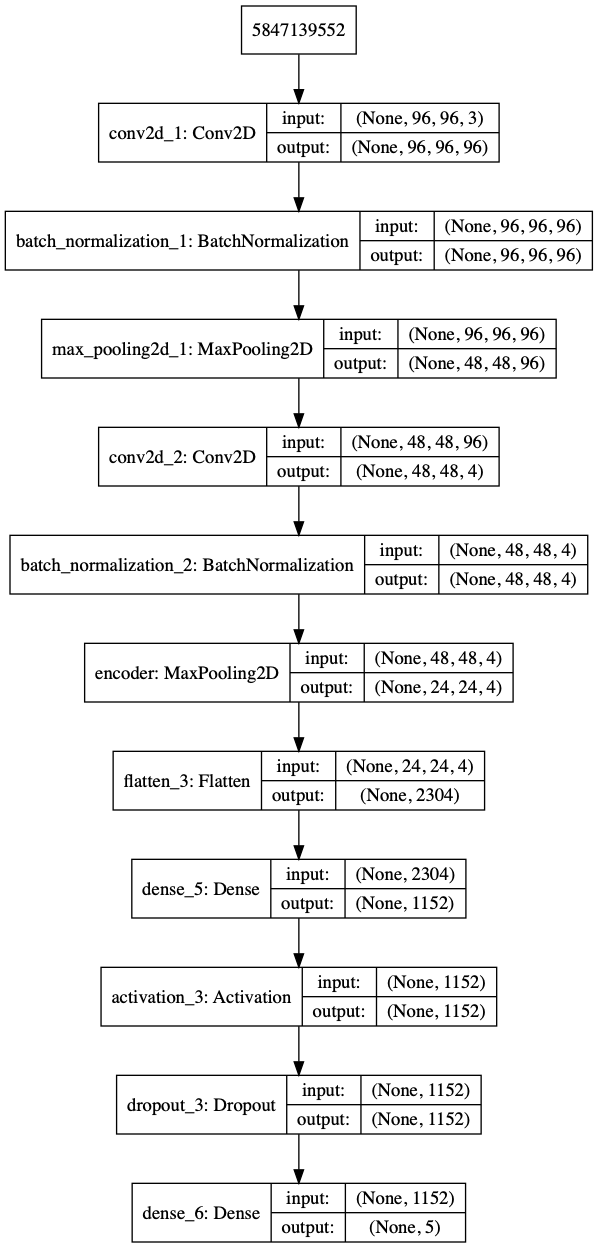
\includegraphics[height=20cm, keepaspectratio]{images/class_architecture}
		\caption{Architecture for classification network. Input and output dimensions $64 \times 64\times3 = 12288$, compression factor 24, encoding dimension 512.}
		\label{fig:class}
	\end{center}
\end{figure}


\paragraph{Architectures} 
The common architecture of the three approaches, apart from the trainability and weight initialization of the parameters, is shown in figure \ref{fig:class}. Several layers are added at the end of the encoder part to allow for classification training. Specifically, the encoded representation is flattened, and passes through two more fully connected layers (Dense layers in Keras). The first of these layers used ReLU, whereas the final layer---containing the classification results---has a sigmoid activation function. Between both layers, dropout is applied. In other words, some of the input to the final layer is dropped out randomly, in an attempt to make the network more robust. The output layer consisted of 5 nodes, to accommodate the K-hot encoded label vector.


\paragraph{Network parameters}
Similar to section \textcolor{blue}{\ref{sec:auto}}, all networks were trained using the \textit{Adam} optimizer algorithm. Several loss functions were experimented with. Results varied, but the comparison between the three presented networks remained fairly consistent. In the remainder of this section, I will discuss results for networks trained using the \textit{binary crossentropy} loss function, as this is the go-to loss function for multi-label classification\footnote{If the problem were multi-class, but not multi-label, the preferred loss function would have been \textit{categorical crossentropy}, combined with a \textit{softmax} activation function in the final layer.}. All model training was set for \textit{300 epochs}. Similar to the approach in section \textcolor{blue}{\ref{sec:auto}}, training stopped if no improvement was detected in the validation loss for a number epochs. After some experimentation, this number was set to 50.

\begin{figure}[!htbp]
	\begin{center}
		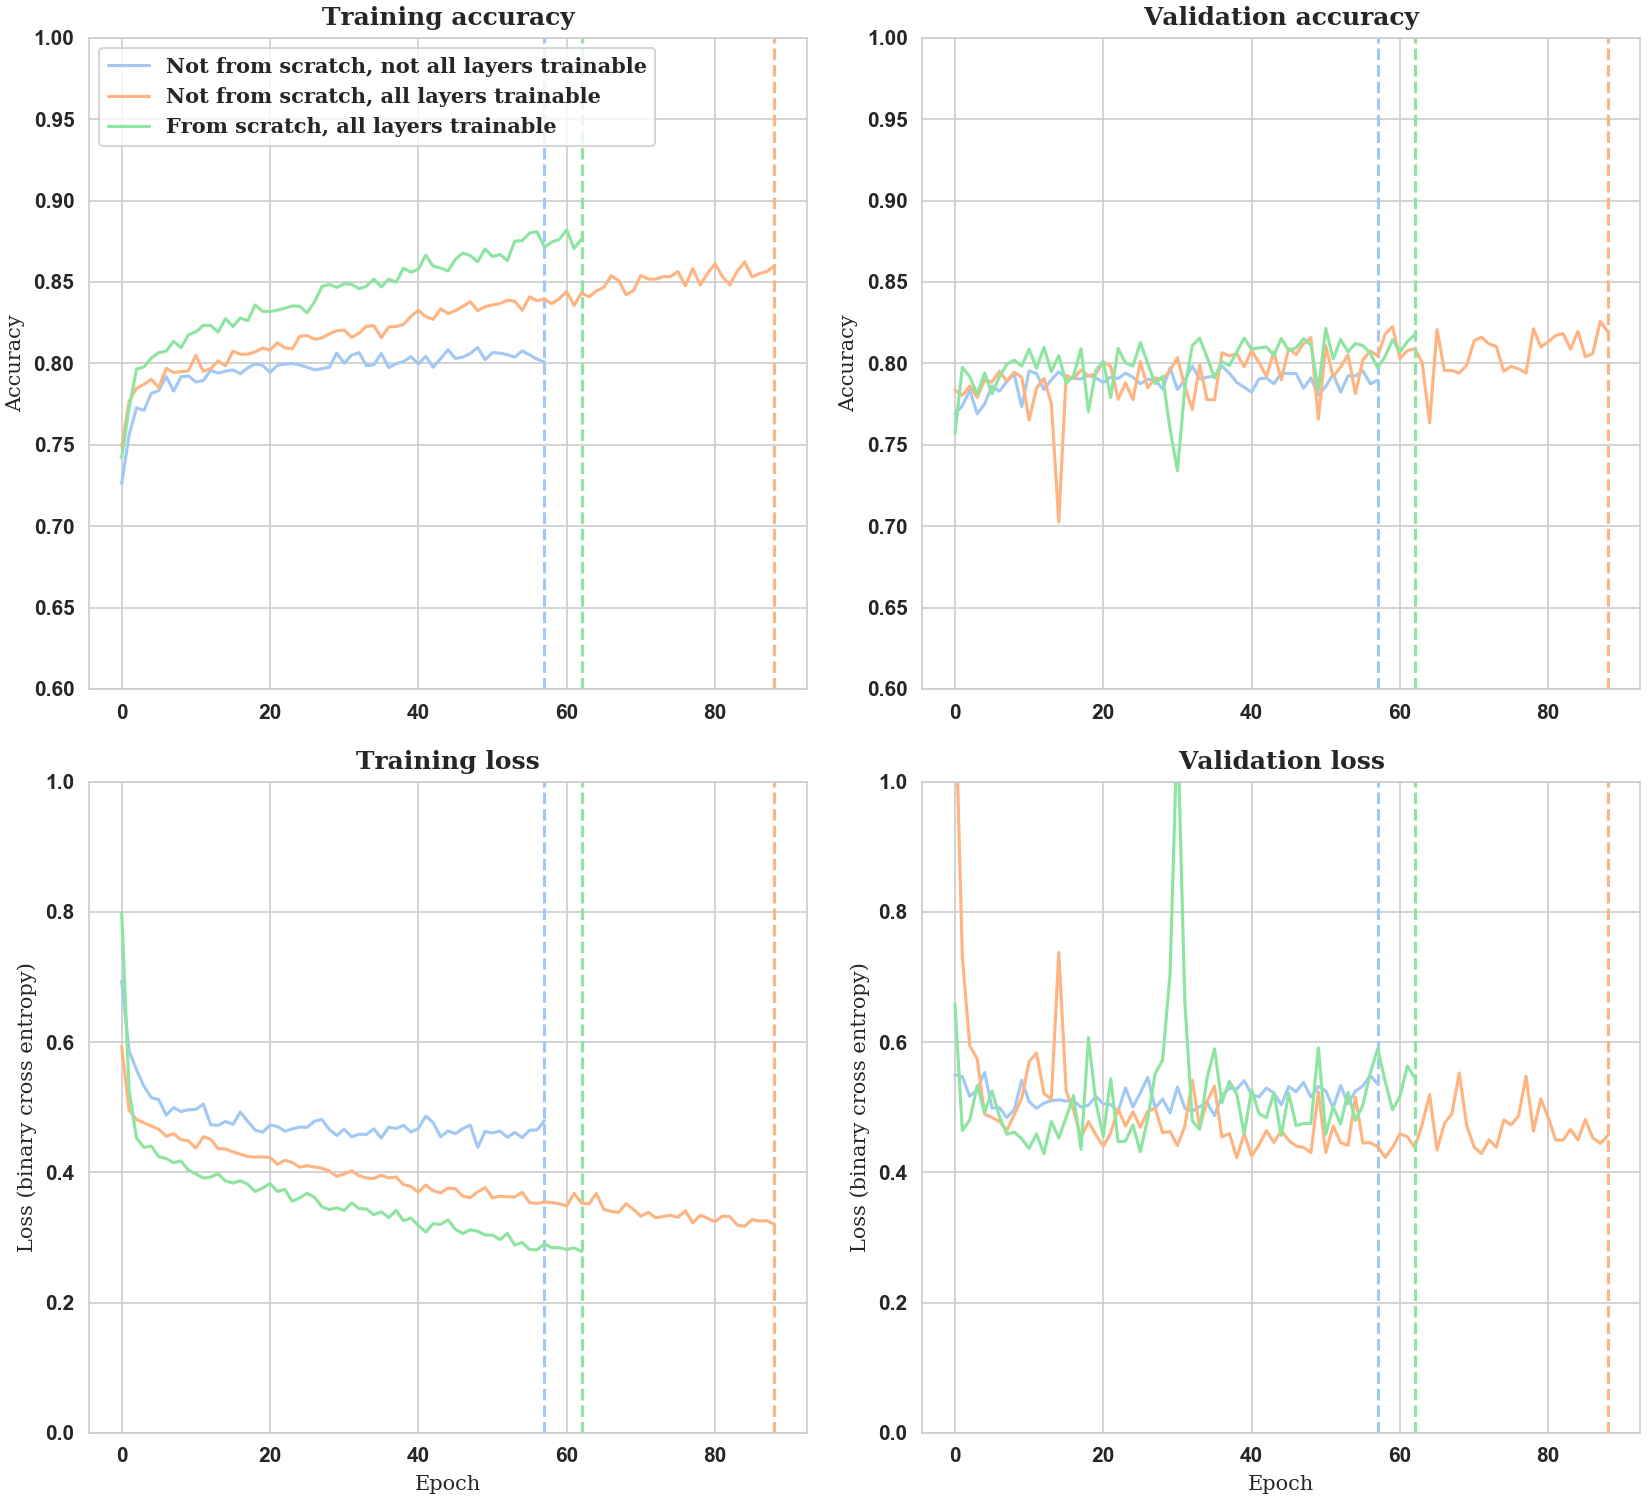
\includegraphics[width=\linewidth, keepaspectratio]{images/class_histories}
		\caption{Training history for all classifier models. In the top row, the left graph shows the evolution of the accuracy on the training data, whereas the right graph shows the evolution of the validation accuracy. In the bottom row, the graphs represent the evolution of the training and validation loss (binary crossentropy). The vertical dotted line indicates when early stopping occurred, due to a lack of improvement in the latter value.}
		\label{fig:class_histories}
	\end{center}
\end{figure}

\paragraph{Evaluation}
%TODO: fix this
All models stopped early re. The bottom left graph in figure \ref{fig:class_histories} shows how training loss decreases steadily for all networks. Unsurprisingly, loss values drop more rapidly in the models with all trainable layers, as these models are more flexible compared to the partially frozen model. The graphs also make clear that training loss would likely have kept decreasing for a significant number of additional epochs. However, judging from the bottom right graph---the validation loss evolution---no real useful information is learnt that applies beyond the training data. 


\subsection{Reflection}
The models presented in this section clearly have limited to no use beyond the training data. There are a several possible explanations for this failure.

\begin{itemize}

	\item{First, it is entirely possible that the model architecture was simply not adequate to capture the relevant information needed to classify the images correctly. If it in fact did succeed in capturing relevant information, then the data compression may have caused the loss of too much necessary information.}
	
	\item{Given the limited number of training images per class (see table \ref{tab:classcounts}), it is possible that the model did not see enough examples to be able to extract recurring semantic features. The problem should therefore probably best be simplified into a binary classification task, to reduce its complexity. Alternatively, additional images could be sought and used as training data (or stolen from the validation set).}

\end{itemize}
